\documentclass{standalone}
\usepackage{tikz}
\usetikzlibrary{patterns, positioning}


\begin{document}
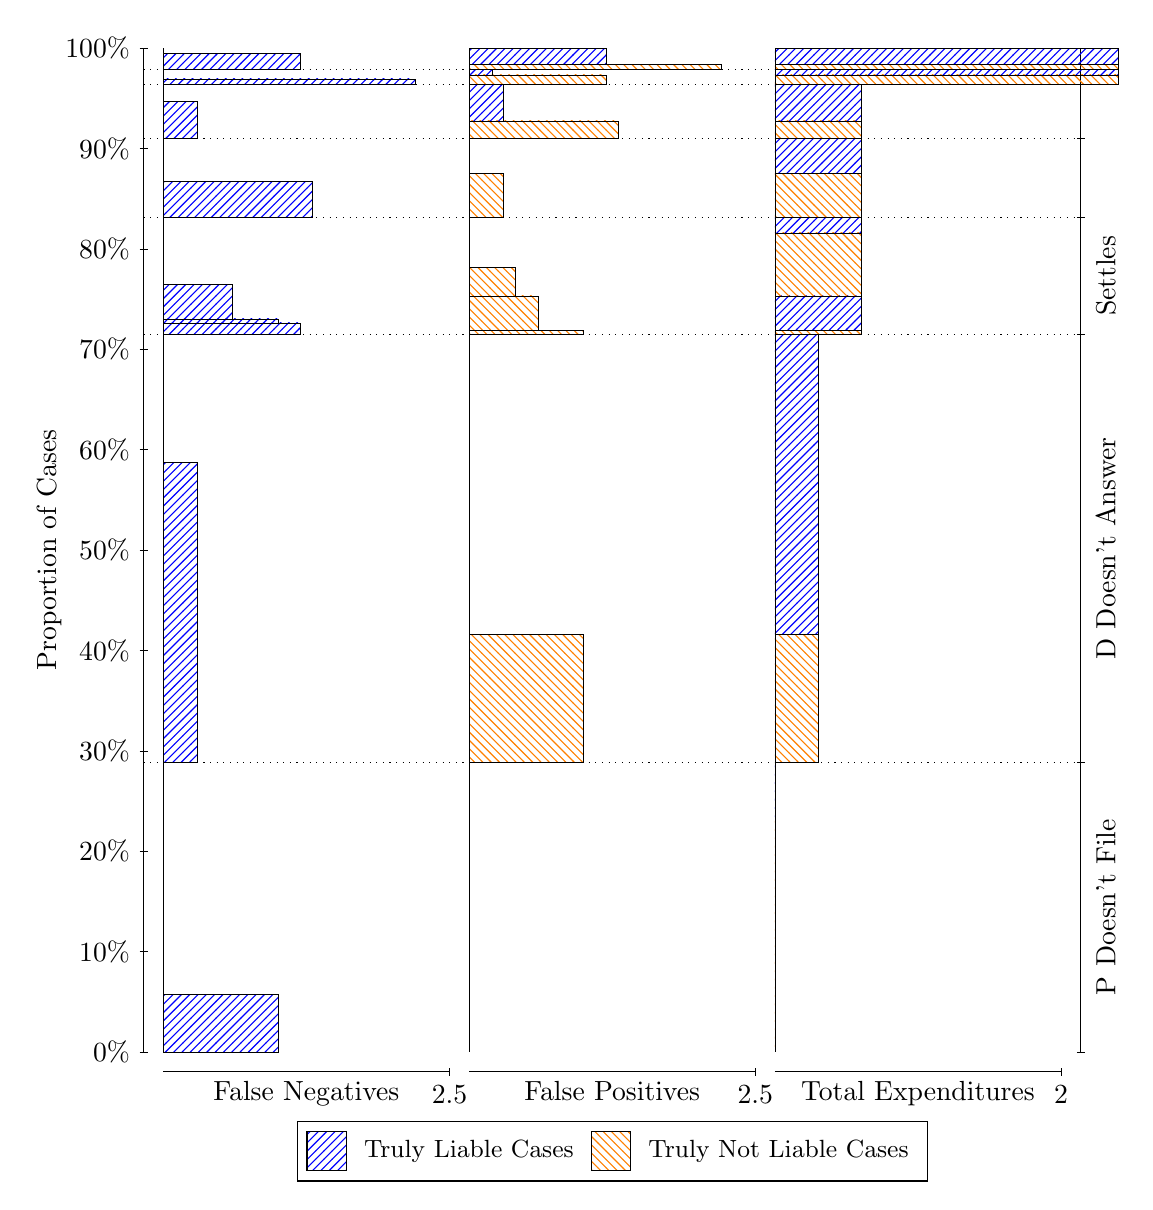
\begin{tikzpicture}
\draw[black, very thin] (1.5,1.75) -- (1.5,14.5);
\node[rotate=90, text=black, anchor=center] at (0.3, 8.125) {Proportion of Cases};
\draw[black, very thin] (1.45,1.75) -- (1.55,1.75);
\node[text=black, anchor=east] at (1.45, 1.75) {0\%};
\draw[black, very thin] (1.45,3.025) -- (1.55,3.025);
\node[text=black, anchor=east] at (1.45, 3.025) {10\%};
\draw[black, very thin] (1.45,4.3) -- (1.55,4.3);
\node[text=black, anchor=east] at (1.45, 4.3) {20\%};
\draw[black, very thin] (1.45,5.575) -- (1.55,5.575);
\node[text=black, anchor=east] at (1.45, 5.575) {30\%};
\draw[black, very thin] (1.45,6.85) -- (1.55,6.85);
\node[text=black, anchor=east] at (1.45, 6.85) {40\%};
\draw[black, very thin] (1.45,8.125) -- (1.55,8.125);
\node[text=black, anchor=east] at (1.45, 8.125) {50\%};
\draw[black, very thin] (1.45,9.4) -- (1.55,9.4);
\node[text=black, anchor=east] at (1.45, 9.4) {60\%};
\draw[black, very thin] (1.45,10.675) -- (1.55,10.675);
\node[text=black, anchor=east] at (1.45, 10.675) {70\%};
\draw[black, very thin] (1.45,11.95) -- (1.55,11.95);
\node[text=black, anchor=east] at (1.45, 11.95) {80\%};
\draw[black, very thin] (1.45,13.225) -- (1.55,13.225);
\node[text=black, anchor=east] at (1.45, 13.225) {90\%};
\draw[black, very thin] (1.45,14.5) -- (1.55,14.5);
\node[text=black, anchor=east] at (1.45, 14.5) {100\%};

\draw[black, very thin] (13.4,1.75) -- (13.4,14.5);
\draw[black, very thin] (13.35,1.75) -- (13.45,1.75);
\node[anchor=west] at (13.35, 1.75) {};
\draw[black, very thin] (13.35,5.4292) -- (13.45,5.4292);
\node[anchor=west] at (13.35, 5.4292) {};
\draw[black, very thin] (13.35,10.86) -- (13.45,10.86);
\node[anchor=west] at (13.35, 10.86) {};
\draw[black, very thin] (13.35,12.352) -- (13.45,12.352);
\node[anchor=west] at (13.35, 12.352) {};
\draw[black, very thin] (13.35,13.356) -- (13.45,13.356);
\node[anchor=west] at (13.35, 13.356) {};
\draw[black, very thin] (13.35,14.041) -- (13.45,14.041);
\node[anchor=west] at (13.35, 14.041) {};
\draw[black, very thin] (13.35,14.227) -- (13.45,14.227);
\node[anchor=west] at (13.35, 14.227) {};
\draw[black, very thin] (13.35,14.5) -- (13.45,14.5);
\node[anchor=west] at (13.35, 14.5) {};

\draw[black, very thin, pattern color=blue, pattern=north east lines] (1.75,1.75) rectangle (3.2033,2.4858);
\draw[black, very thin, pattern color=orange, pattern=north west lines] (1.75,2.4858) rectangle (1.75,5.4292);
\draw[black, very thin, pattern color=blue, pattern=north east lines] (1.75,5.4292) rectangle (2.186,9.2379);
\draw[black, very thin, pattern color=orange, pattern=north west lines] (1.75,9.2379) rectangle (1.75,10.86);
\draw[black, very thin, pattern color=blue, pattern=north east lines] (1.75,10.86) rectangle (3.494,11.01);
\draw[black, very thin, pattern color=blue, pattern=north east lines] (1.75,11.01) rectangle (3.2033,11.061);
\draw[black, very thin, pattern color=blue, pattern=north east lines] (1.75,11.061) rectangle (2.622,11.501);
\draw[black, very thin, pattern color=orange, pattern=north west lines] (1.75,11.501) rectangle (1.75,12.352);
\draw[black, very thin, pattern color=blue, pattern=north east lines] (1.75,12.352) rectangle (3.6393,12.803);
\draw[black, very thin, pattern color=orange, pattern=north west lines] (1.75,12.803) rectangle (1.75,13.356);
\draw[black, very thin, pattern color=blue, pattern=north east lines] (1.75,13.356) rectangle (2.186,13.822);
\draw[black, very thin, pattern color=orange, pattern=north west lines] (1.75,13.822) rectangle (1.75,14.041);
\draw[black, very thin, pattern color=blue, pattern=north east lines] (1.75,14.041) rectangle (4.9473,14.109);
\draw[black, very thin, pattern color=orange, pattern=north west lines] (1.75,14.109) rectangle (1.75,14.227);
\draw[black, very thin, pattern color=blue, pattern=north east lines] (1.75,14.227) rectangle (3.494,14.431);
\draw[black, very thin, pattern color=orange, pattern=north west lines] (1.75,14.431) rectangle (1.75,14.5);
\draw[black, very thin, pattern color=orange, pattern=north west lines] (5.6333,1.75) rectangle (5.6333,4.6933);
\draw[black, very thin, pattern color=blue, pattern=north east lines] (5.6333,4.6933) rectangle (5.6333,5.4292);
\draw[black, very thin, pattern color=orange, pattern=north west lines] (5.6333,5.4292) rectangle (7.0867,7.0508);
\draw[black, very thin, pattern color=blue, pattern=north east lines] (5.6333,7.0508) rectangle (5.6333,10.86);
\draw[black, very thin, pattern color=orange, pattern=north west lines] (5.6333,10.86) rectangle (7.0867,10.911);
\draw[black, very thin, pattern color=orange, pattern=north west lines] (5.6333,10.911) rectangle (6.5053,11.351);
\draw[black, very thin, pattern color=orange, pattern=north west lines] (5.6333,11.351) rectangle (6.2147,11.711);
\draw[black, very thin, pattern color=blue, pattern=north east lines] (5.6333,11.711) rectangle (5.6333,12.352);
\draw[black, very thin, pattern color=orange, pattern=north west lines] (5.6333,12.352) rectangle (6.0693,12.906);
\draw[black, very thin, pattern color=blue, pattern=north east lines] (5.6333,12.906) rectangle (5.6333,13.356);
\draw[black, very thin, pattern color=orange, pattern=north west lines] (5.6333,13.356) rectangle (7.5227,13.575);
\draw[black, very thin, pattern color=blue, pattern=north east lines] (5.6333,13.575) rectangle (6.0693,14.041);
\draw[black, very thin, pattern color=orange, pattern=north west lines] (5.6333,14.041) rectangle (7.3773,14.158);
\draw[black, very thin, pattern color=blue, pattern=north east lines] (5.6333,14.158) rectangle (5.924,14.227);
\draw[black, very thin, pattern color=orange, pattern=north west lines] (5.6333,14.227) rectangle (8.8307,14.296);
\draw[black, very thin, pattern color=blue, pattern=north east lines] (5.6333,14.296) rectangle (7.3773,14.5);
\draw[black, very thin, pattern color=orange, pattern=north west lines] (9.5167,1.75) rectangle (9.5167,4.6933);
\draw[black, very thin, pattern color=blue, pattern=north east lines] (9.5167,4.6933) rectangle (9.5167,5.4292);
\draw[black, very thin, pattern color=orange, pattern=north west lines] (9.5167,5.4292) rectangle (10.062,7.0508);
\draw[black, very thin, pattern color=blue, pattern=north east lines] (9.5167,7.0508) rectangle (10.062,10.86);
\draw[black, very thin, pattern color=orange, pattern=north west lines] (9.5167,10.86) rectangle (10.607,10.911);
\draw[black, very thin, pattern color=blue, pattern=north east lines] (9.5167,10.911) rectangle (10.607,11.351);
\draw[black, very thin, pattern color=orange, pattern=north west lines] (9.5167,11.351) rectangle (10.607,12.151);
\draw[black, very thin, pattern color=blue, pattern=north east lines] (9.5167,12.151) rectangle (10.607,12.352);
\draw[black, very thin, pattern color=orange, pattern=north west lines] (9.5167,12.352) rectangle (10.607,12.906);
\draw[black, very thin, pattern color=blue, pattern=north east lines] (9.5167,12.906) rectangle (10.607,13.356);
\draw[black, very thin, pattern color=orange, pattern=north west lines] (9.5167,13.356) rectangle (10.607,13.575);
\draw[black, very thin, pattern color=blue, pattern=north east lines] (9.5167,13.575) rectangle (10.607,14.041);
\draw[black, very thin, pattern color=orange, pattern=north west lines] (9.5167,14.041) rectangle (13.877,14.158);
\draw[black, very thin, pattern color=blue, pattern=north east lines] (9.5167,14.158) rectangle (13.877,14.227);
\draw[black, very thin, pattern color=orange, pattern=north west lines] (9.5167,14.227) rectangle (13.877,14.296);
\draw[black, very thin, pattern color=blue, pattern=north east lines] (9.5167,14.296) rectangle (13.877,14.5);
\draw[black, dotted] (1.5,5.4292) -- (13.4,5.4292);
\draw[black, dotted] (1.5,10.86) -- (13.4,10.86);
\draw[black, dotted] (1.5,12.352) -- (13.4,12.352);
\draw[black, dotted] (1.5,13.356) -- (13.4,13.356);
\draw[black, dotted] (1.5,14.041) -- (13.4,14.041);
\draw[black, dotted] (1.5,14.227) -- (13.4,14.227);
\draw[black, very thin] (1.75,1.5) -- (5.3833,1.5);
\node[text=black, anchor=north] at (3.5667, 1.5) {False Negatives};
\draw[black, very thin] (5.3833,1.45) -- (5.3833,1.55);
\node[text=black, anchor=north] at (5.3833, 1.45) {2.5};

\draw[black, very thin] (5.6333,1.5) -- (9.2667,1.5);
\node[text=black, anchor=north] at (7.45, 1.5) {False Positives};
\draw[black, very thin] (9.2667,1.45) -- (9.2667,1.55);
\node[text=black, anchor=north] at (9.2667, 1.45) {2.5};

\draw[black, very thin] (9.5167,1.5) -- (13.15,1.5);
\node[text=black, anchor=north] at (11.333, 1.5) {Total Expenditures};
\draw[black, very thin] (13.15,1.45) -- (13.15,1.55);
\node[text=black, anchor=north] at (13.15, 1.45) {2};

\node[text=black, centered, rotate=90] at (13.72, 3.5896) {P Doesn't File};
\node[text=black, centered, rotate=90] at (13.72, 8.1444) {D Doesn't Answer};
\node[text=black, centered, rotate=90] at (13.72, 11.606) {Settles};





\draw (7.449999999999999,1.5) node[draw=none] (baseCoordinate) {};
\begin{scope}[align=center]
        \matrix[scale=0.5, draw=black, below=0.5cm of baseCoordinate, nodes={draw}, column sep=0.1cm]{
            \node[rectangle, draw, minimum width=0.5cm, minimum height=0.5cm, pattern color=blue, pattern=north east lines] {}; &
            \node[draw=none, font=\small, text=black] (B) {Truly Liable Cases}; &
            \node[rectangle, draw, minimum width=0.5cm, minimum height=0.5cm, pattern color=orange, pattern=north west lines] {}; &
            \node[draw=none, font=\small, text=black] (B) {Truly Not Liable Cases}; \\
            };
\end{scope}

\end{tikzpicture}
\end{document}